\chapter{Genomika dan Pengurutan}\label{ch:b3:genomics}

Genom lengkap pertama sebuah organisme yang hidup bebas, yaitu \qty{1.8}{Mb}
milik sebuah bakteri, diterbitkan pada tahun 1995 sesudah setahun kerja sebuah
tim beranggota empat puluh orang. Genom manusia, \num{3.2} miliar pasangan
basa, menghabiskan tiga belas tahun kerja sebuah konsorsium internasional dan
kira-kira tiga miliar dolar, lalu dinyatakan rampung pada tahun 2003. Kini
sebuah mesin meja membaca genom manusia dalam semalam dengan biaya beberapa
ratus dolar, sebuah rumah sakit mengurutkan tumor seorang pasien untuk memilih
obat, dan sebuah museum mengekstraksi lalu membaca genom sepotong tulang
berumur empat puluh ribu tahun. Teknologi yang memungkinkan semua itu,
matematika yang mengubah jutaan \omterm{def:b3:genomics:ngs}{bacaan} pendek menjadi sebuah genom, dan apa
yang diajarkan genom yang telah rampung tentang ukuran, isi, serta sejarah DNA
kita adalah pokok bab ini. Bab sesudahnya membahas algoritma yang
membandingkan urutannya begitu urutan itu ada di tangan.

\section{Membaca DNA}

\begin{definition}[Pengurutan lewat penghentian rantai]\label{def:b3:genomics:sanger}
\index{pengurutan Sanger}\index{dideoksinukleotida}\index{penghentian rantai}
\emph{Pengurutan Sanger} menyalin cetakan beruntai tunggal mulai dari sebuah
primer dengan DNA polimerase, dengan kehadiran keempat nukleotida normal dan
sedikit \emph{dideoksinukleotida}, yang tidak memiliki hidroksil 3$'$ sehingga
menghentikan rantainya di mana pun ia disisipkan. Tiap dideoksinukleotida
mengusung zat warna berpendar yang berbeda. Hasilnya berupa campuran fragmen,
satu fragmen bagi tiap kedudukan cetakannya, yang masing-masing berakhir pada
basa yang jati dirinya diketahui; setelah dipisahkan menurut ukurannya di
dalam kapiler gel, fragmen itu melewati detektor berurutan menurut panjangnya,
dan deretan warnanya adalah urutan cetakannya. Sekali jalan terbaca
\qtyrange{700}{900}{bp} dengan laju galat di bawah $10^{-3}$; cara ini tetap
dipakai untuk memastikan sebuah konstruk atau satu gen.
\end{definition}

\begin{proof}[Bukti eksperimental]
Sanger, Nicklen, dan Coulson menerbitkan metodenya pada tahun 1977 lalu
memakainya pada tahun itu juga untuk membaca \qty{5386}{bp} fag $\phi$X174 ---
genom DNA lengkap yang pertama --- dan pada tahun 1981 membaca \qty{16569}{bp}
mitokondria manusia. Fleischmann dan rekan (1995) membaca
\qty{1.83}{Mb} \emph{Haemophilus influenzae} dengan memecah seluruh
genomnya menjadi fragmen acak, mengurutkan \num{24000} di antaranya, lalu
merakit \omterm{def:b3:genomics:ngs}{bacaannya} dengan komputer --- strategi \emph{senapan seluruh genom}
yang diperbesar setiap proyek berikutnya.
\end{proof}

\begin{omfigure}
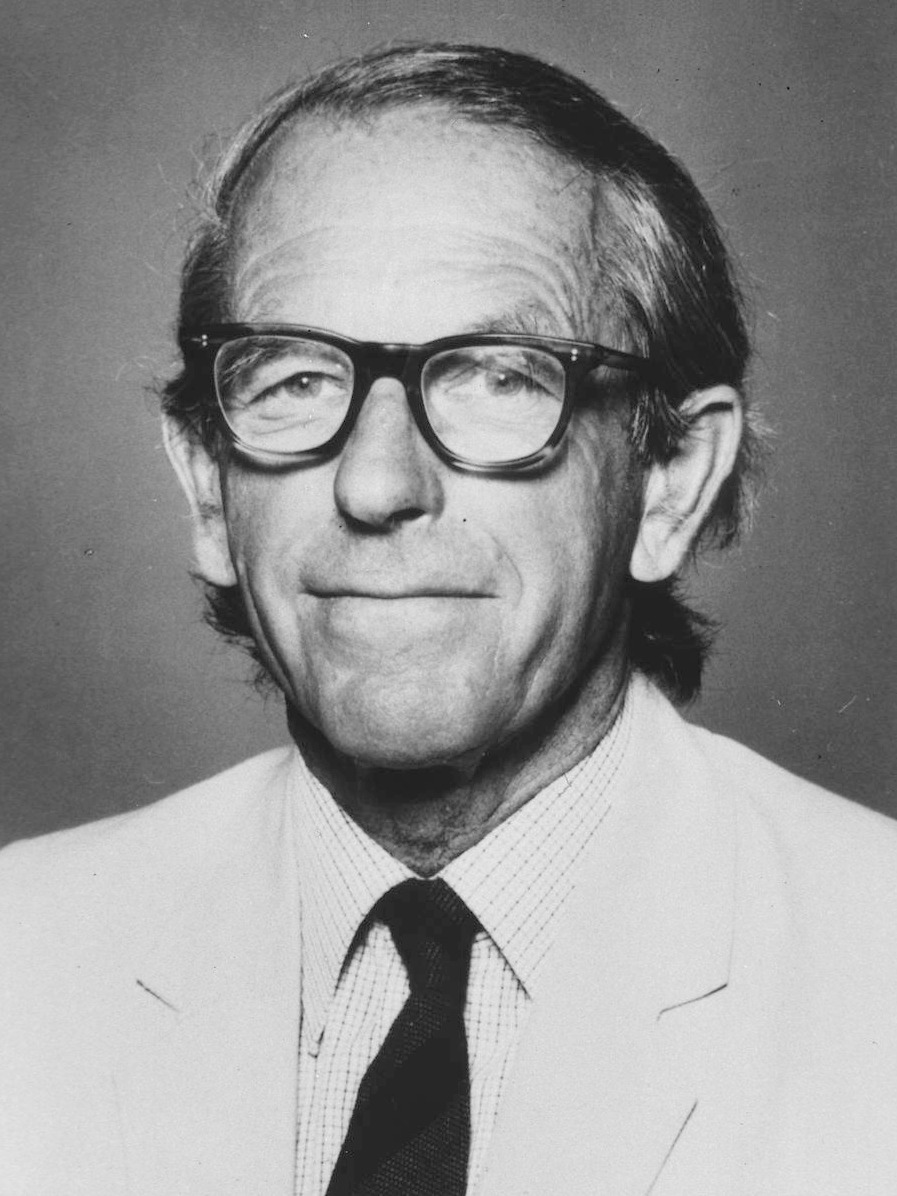
\includegraphics[width=0.30\linewidth]{images/book5/sanger.jpg}\hspace{0.04\linewidth}
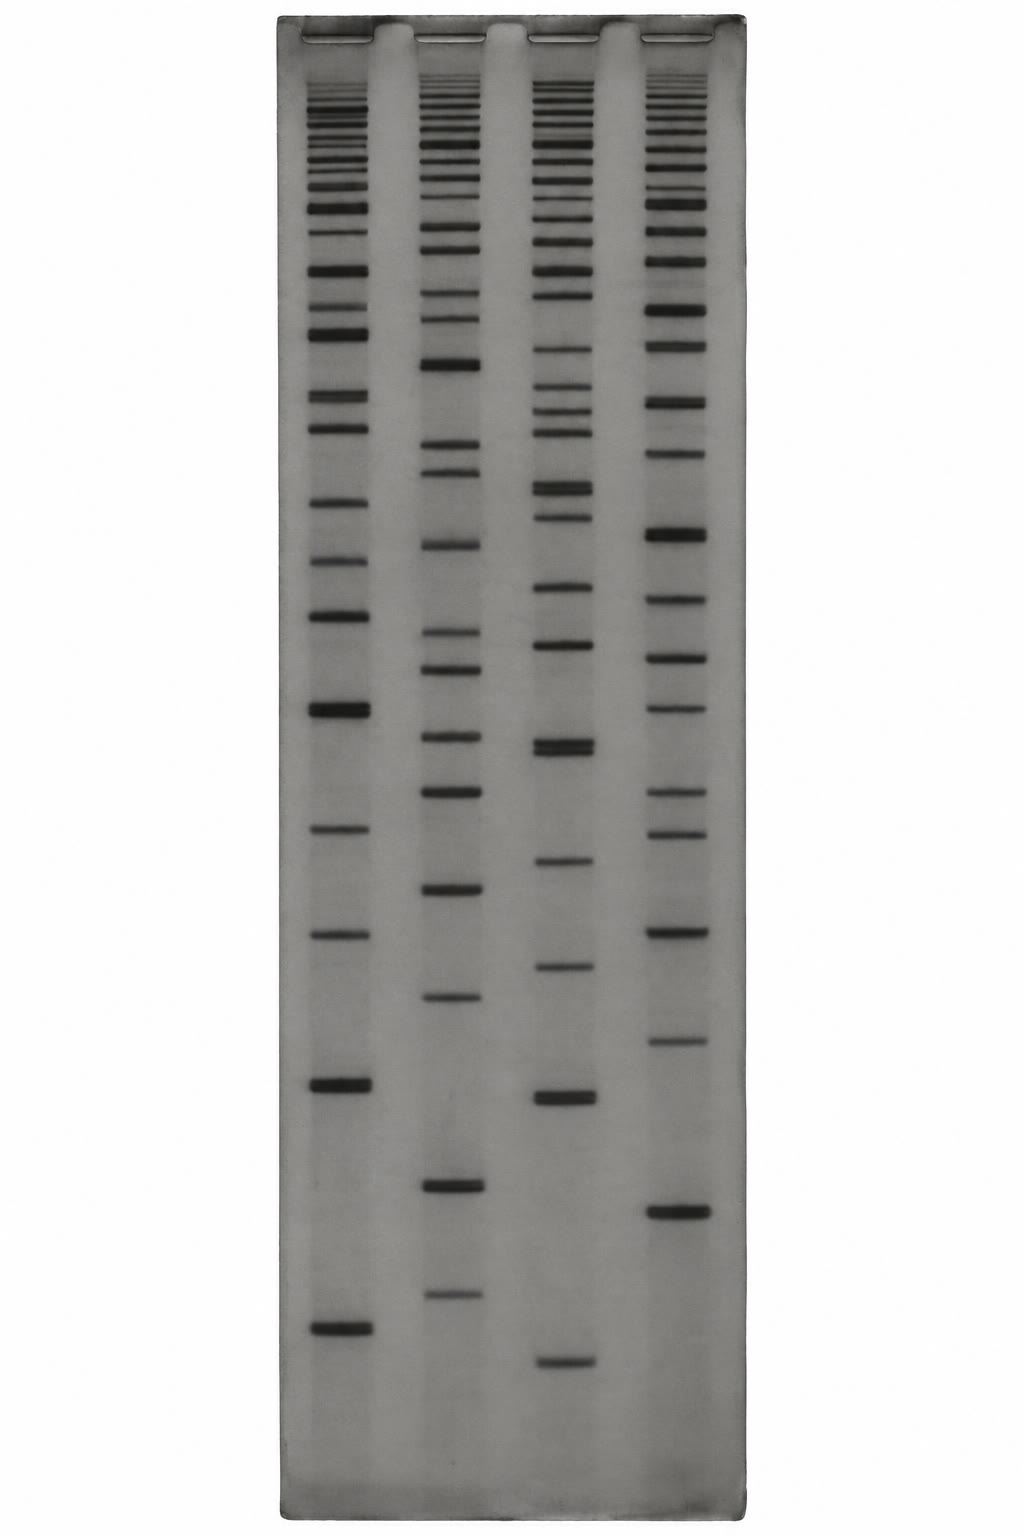
\includegraphics[width=0.30\linewidth]{images/book5/ai/b5-04-sanger-gel.jpg}

{\small Kiri: Frederick Sanger, yang merancang metode praktis pertama untuk
membaca protein dan DNA serta menerima hadiah Nobel untuk masing-masing.
Kanan: autoradiograf sebuah gel pengurutan dari zaman sebelum kapiler, satu
jalur tiap basa, urutannya dibaca ke atas dari tangga pitanya.}
\end{omfigure}

\begin{omfigure}
\begin{tikzpicture}[every node/.style={font=\scriptsize}, >=stealth]
  % template and primer
  \draw[very thick, omDef] (0,3.0) -- (6,3.0); \node[left] at (-0.1,3.0) {cetakan 3$'$};
  \node[right] at (6.05,3.0) {5$'$};
  \foreach \x/\b in {0.6/T,1.2/G,1.8/A,2.4/C,3.0/T,3.6/T,4.2/G,4.8/C} \node[above, omDef] at (\x,3.05) {\b};
  \draw[very thick, omProp] (0,2.6) -- (0.3,2.6); \node[left] at (-0.1,2.6) {pemula};
  % terminated products
  \foreach \i/\len/\col/\b in {1/0.6/omDef/A, 2/1.2/omMeth/C, 3/1.8/omThm/T, 4/2.4/omExo/G, 5/3.0/omDef/A, 6/3.6/omDef/A, 7/4.2/omMeth/C, 8/4.8/omExo/G} {
    \draw[very thick, omProp] (0,2.6-0.32*\i) -- (\len-0.15,2.6-0.32*\i);
    \fill[\col] (\len-0.05,2.6-0.32*\i) circle (0.1);
    \node[right, \col] at (\len+0.05,2.6-0.32*\i) {dd\b};
  }
  \node[below, align=center] at (2.4,-0.25) {satu hasil bagi tiap kedudukan, masing-masing berakhir\\pada basa dideoksi berpendar};
  % capillary readout
  \draw[->, thick] (6.5,1.3) -- (7.4,1.3) node[midway, above] {ukuran};
  \draw[thick] (7.6,0.0) rectangle (11.6,2.6);
  \foreach \i/\col in {1/omDef, 2/omMeth, 3/omThm, 4/omExo, 5/omDef, 6/omDef, 7/omMeth, 8/omExo} {
    \draw[very thick, \col] (7.6+0.45*\i,0.1) .. controls (7.6+0.45*\i-0.15,0.1) and (7.6+0.45*\i-0.1,1.6) .. (7.6+0.45*\i,1.6) .. controls (7.6+0.45*\i+0.1,1.6) and (7.6+0.45*\i+0.15,0.1) .. (7.6+0.45*\i+0.3,0.1);
  }
  \foreach \i/\b in {1/A, 2/C, 3/T, 4/G, 5/A, 6/A, 7/C, 8/G} \node[above] at (7.6+0.45*\i,1.7) {\b};
  \node[below] at (9.6,-0.05) {terpendek $\to$ terpanjang: urutannya, dibaca lewat warna};
\end{tikzpicture}

{\small Pengurutan lewat \omterm{def:b3:genomics:sanger}{penghentian rantai}. Sebuah basa dideoksi mengakhiri
salinannya pada tiap kedudukan tempat ia disisipkan; fragmennya, satu tiap
panjang, dipisahkan menurut ukuran, lalu warna tiap basa ujungnya dibaca
berurutan.}
\end{omfigure}

\begin{definition}[Pengurutan paralel besar-besaran]\label{def:b3:genomics:ngs}
\index{pengurutan lewat sintesis}\index{bacaan}%
\index{pengurutan bacaan panjang}\index{nanopori}
Instrumen generasi kedua membaca jutaan sampai miliaran fragmen sekaligus.
Pada \emph{pengurutan lewat sintesis}, fragmennya, yang ujungnya telah diligasi
dengan adaptor, diikatkan pada sel alir kaca lalu diperbanyak di tempat
menjadi gugusan molekul yang identik; gugusan itu lalu dipanjangkan satu basa
tiap daur dengan nukleotida berpendar yang terblokir secara berbalik, dicitra,
dibuka bloknya, lalu dipanjangkan lagi, sehingga tiap daur menambahkan satu
basa pada \emph{bacaan} setiap gugusan. Bacaannya sepanjang
\qtyrange{100}{300}{bp}, biasanya dari kedua ujung sebuah fragmen
(\emph{ujung berpasangan}), dengan laju galat kira-kira $10^{-3}$ tiap basa,
dan sekali jalan menghasilkan sampai $10^{12}$ basa. Instrumen
\emph{bacaan panjang} generasi ketiga membaca molekul tunggal tanpa
perbanyakan: dengan mengamati satu polimerase menyisipkan nukleotida berpendar
secara waktu nyata, atau dengan menyusupkan DNA-nya melalui \emph{nanopori}
protein lalu merekam arus ionnya, yang dimodulasi tiap urutan basa dengan
caranya sendiri. Bacaan sepanjang \qtyrange{10}{100}{kb} dan lebih melintasi
urutan berulang yang tak terjangkau bacaan pendek, dengan laju galat mentah
yang lebih tinggi tetapi dikurangi oleh konsensus.
\end{definition}

\begin{omfigure}
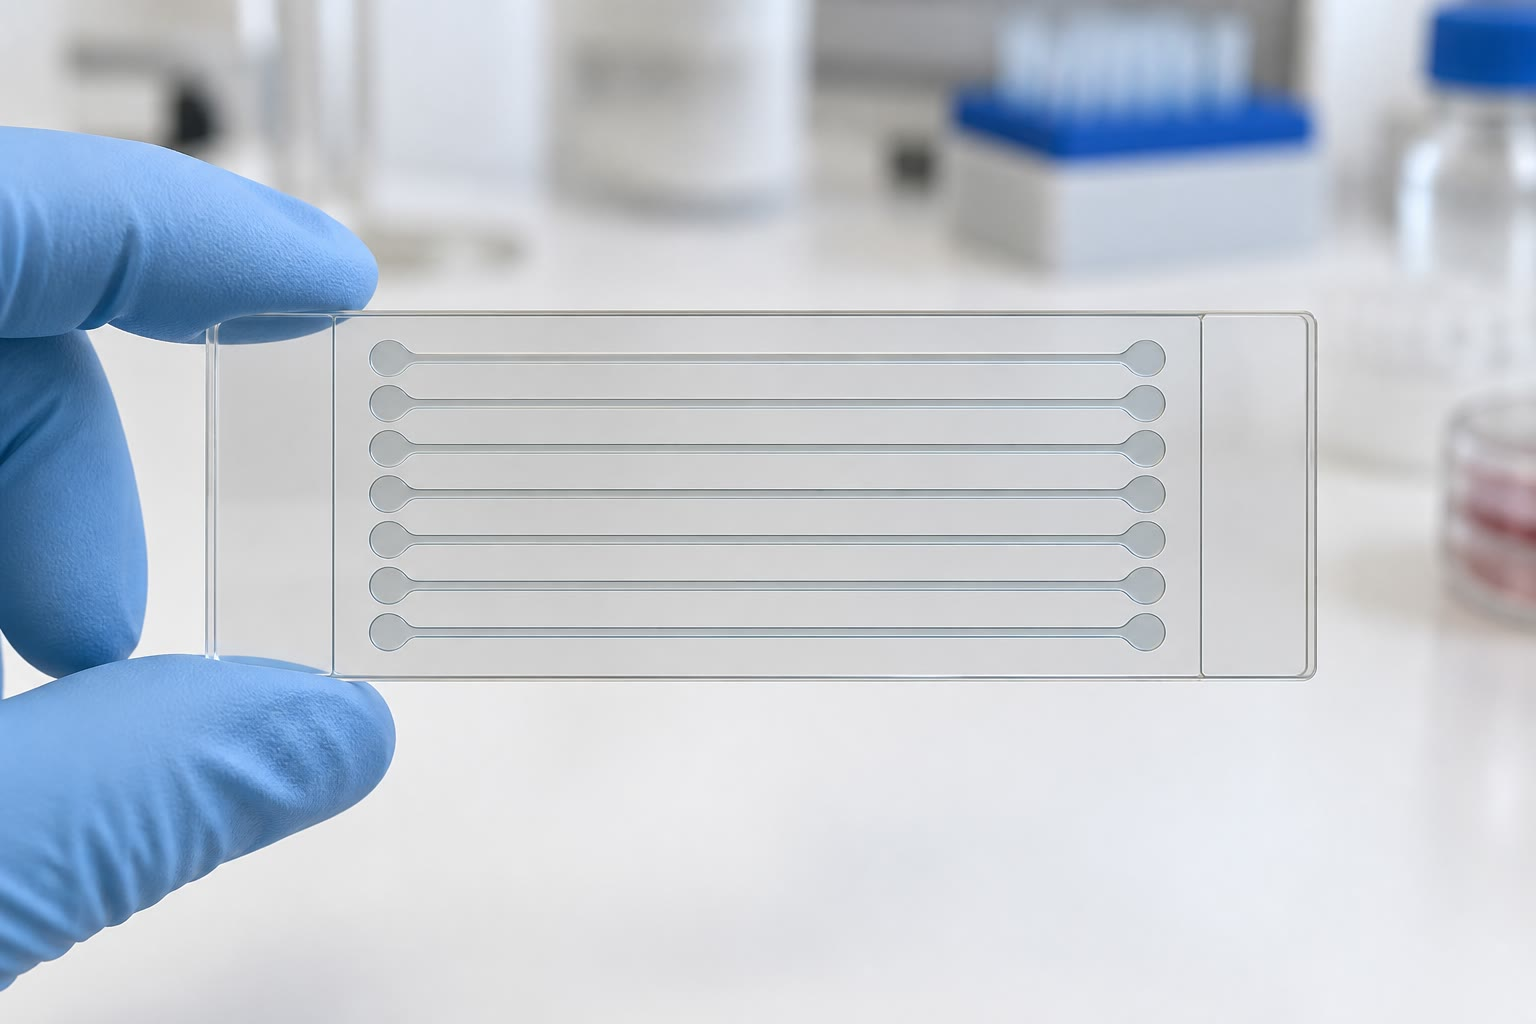
\includegraphics[width=0.46\linewidth]{images/book5/ai/b5-04-flowcell.jpg}\hspace{0.04\linewidth}
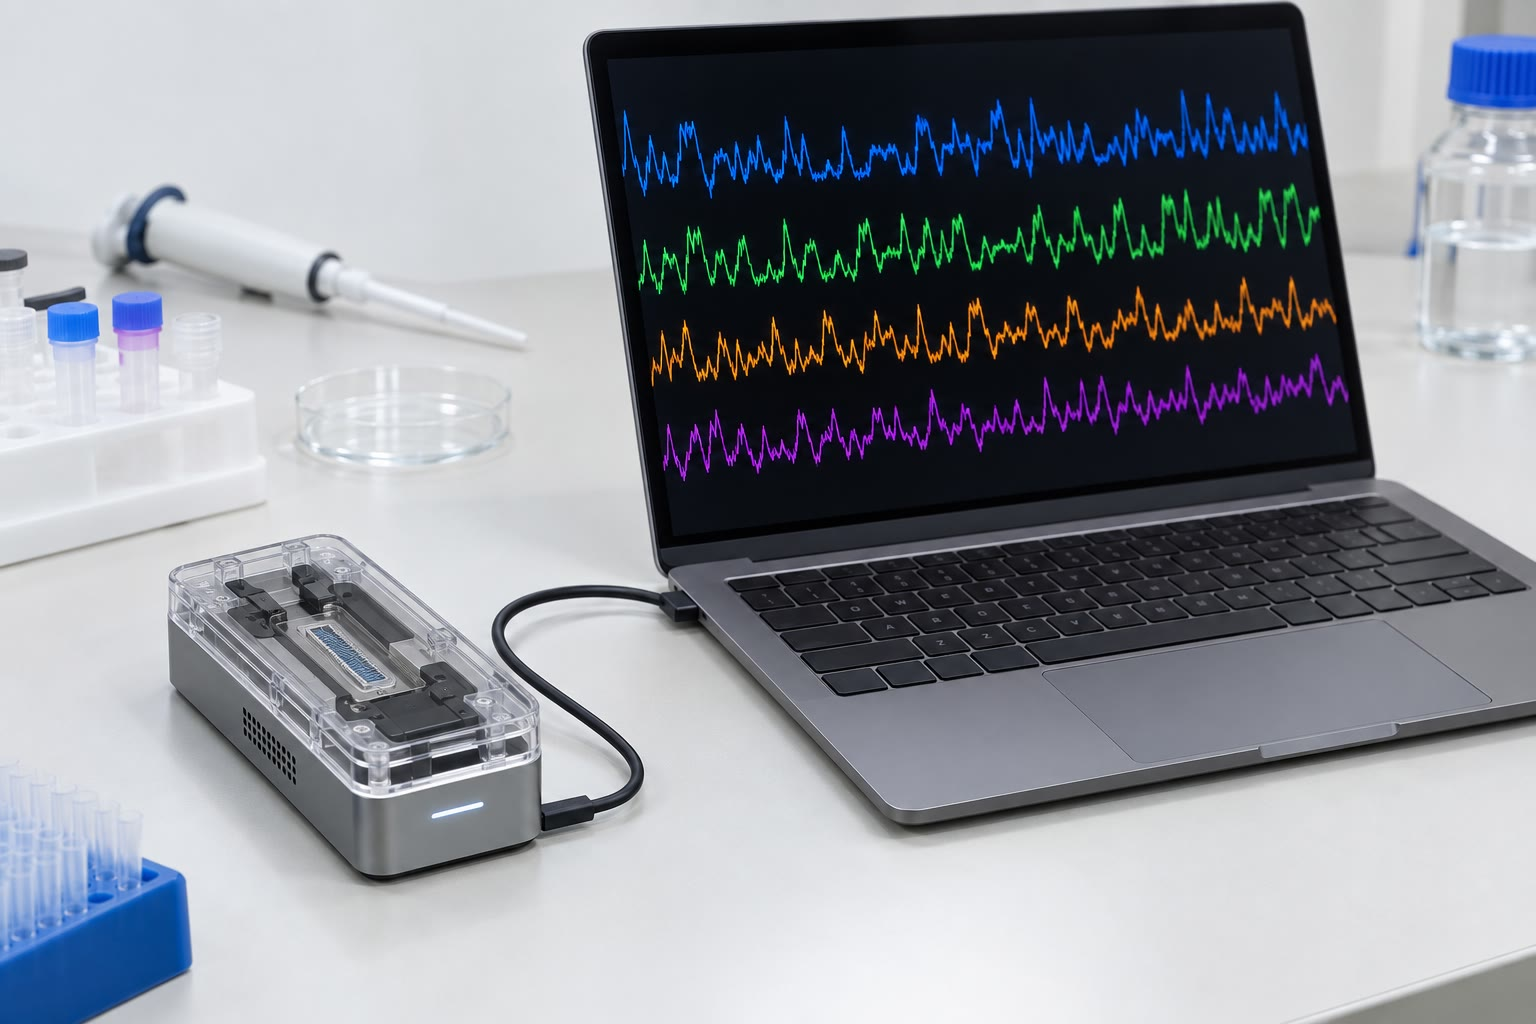
\includegraphics[width=0.46\linewidth]{images/book5/ai/b5-04-nanopore.jpg}

{\small Kiri: sebuah sel alir, yaitu kaca preparat tempat miliaran gugusan
DNA ditumbuhkan lalu dibaca satu basa tiap daur. Kanan: sebuah pengurut
\omterm{def:b3:genomics:ngs}{nanopori} sebesar saku yang membaca molekul tunggal sebagai perubahan arus
ion.}
\end{omfigure}

\begin{theorem}[Cakupan dan celah dalam proyek senapan]\label{thm:b3:genomics:lander-waterman}
\index{cakupan}\index{Lander--Waterman}\index{kontig}
Misalkan $N$ \omterm{def:b3:genomics:ngs}{bacaan} sepanjang $L$ diambil pada kedudukan acak sepanjang
genom sepanjang $G$, dan misalkan $c = NL/G$ adalah \emph{cakupan}, yakni
rata-rata cacah \omterm{def:b3:genomics:ngs}{bacaan} yang meliputi satu basa. Maka sebuah basa tertentu
diliputi oleh cacah \omterm{def:b3:genomics:ngs}{bacaan} yang tersebar Poisson dengan rata-rata $c$: bagian
genom yang tak terurutkan adalah
\[
P(\text{tak tercakup}) = e^{-c},
\]
dan bila dua \omterm{def:b3:genomics:ngs}{bacaan} diakui bertindihan hanya ketika keduanya berbagi
sedikitnya $T$ basa, sehingga $\theta = T/L$, harapan cacah
\emph{kontig} (pulau \omterm{def:b3:genomics:ngs}{bacaan} yang bertindihan) adalah
\[
\text{kontig} = N\,e^{-c(1-\theta)},
\]
dan panjang rata-ratanya kira-kira $L\,\bigl(e^{c(1-\theta)} - 1\bigr)/c + L\theta$.
\end{theorem}
\begin{proof}
Titik awal \omterm{def:b3:genomics:ngs}{bacaan} jatuh secara acak dengan kerapatan $N/G$ tiap basa. Sebuah
basa diliputi \omterm{def:b3:genomics:ngs}{bacaan} yang mulai pada $L$ basa sebelumnya; cacah awalan di
dalam jendela sepanjang $L$ tersebar Poisson dengan rata-rata $LN/G
= c$, dan peluang tanpa satu pun awalan adalah $e^{-c}$. Sebuah \omterm{def:b3:genomics:ngs}{bacaan} menjadi
\omterm{def:b3:genomics:ngs}{bacaan} paling kanan pada kontignya bila tak ada \omterm{def:b3:genomics:ngs}{bacaan} lain yang mulai di
dalam $L - T = L(1-\theta)$ basa sesudah awalannya sendiri (\omterm{def:b3:genomics:ngs}{bacaan} yang mulai
lebih lambat akan bertindihan dengannya kurang dari $T$ sehingga tak
disambungkan); peluangnya adalah $e^{-c(1-\theta)}$, dan karena tiap kontig
memiliki tepat satu \omterm{def:b3:genomics:ngs}{bacaan} paling kanan, harapan cacah kontignya adalah
$N e^{-c(1-\theta)}$. Panjang kontig rata-ratanya menyusul dari $G$ dibagi
cacah kontignya, dengan koreksi bagi bagian yang tak terliput.
\end{proof}

\begin{example}[Berapa yang memadai]\label{ex:b3:genomics:coverage}
Pada $c = 5$ bagian yang tak terurutkan adalah $e^{-5} = 0.7\,\%$ --- bagi
genom \qty{3.2}{Gb}, dua puluh juta basa di dalam beberapa puluh ribu celah.
Pada $c = 10$ bagian itu $4.5\times 10^{-5}$, seluruhnya \qty{150}{kb}.
Genom manusia lazimnya diurutkan pada $c = 30$ bukan karena celah cakupannya
($e^{-30} \approx 10^{-13}$) melainkan karena tiap basa harus dibaca beberapa
kali pada masing-masing dari kedua kromosomnya agar varian heterozigot dapat
dipanggil dengan yakin melawan laju galat $10^{-3}$ tiap \omterm{def:b3:genomics:ngs}{bacaan}. Genom
bakteri diurutkan pada $c = 50$--$100$ karena alasan yang sama dan karena
biayanya murah. Rumusnya juga memperlihatkan apa yang tak dapat diperbaiki
cakupan: urutan berulang yang lebih panjang daripada sebuah \omterm{def:b3:genomics:ngs}{bacaan} adalah
tempat graf pertindihannya bercabang, dan sebanyak apa pun \omterm{def:b3:genomics:ngs}{bacaan} pendek tak
dapat menguraikannya. Untuk itulah \omterm{def:b3:genomics:ngs}{bacaan} panjang ada.
\end{example}

\begin{omfigure}
\begin{tikzpicture}
\begin{axis}[
  width=0.7\linewidth, height=5.6cm,
  axis x line=bottom, axis y line=left,
  xmin=0, xmax=12, ymin=0.000001, ymax=1, ymode=log,
  xlabel={cakupan $c$}, ylabel={bagian},
  xlabel style={font=\small, at={(axis description cs:0.5,-0.12)}, anchor=north},
  ylabel style={font=\small},
  tick label style={font=\small}, xtick={0,2,4,6,8,10,12},
  clip=false,
]
\addplot[very thick, omDef, domain=0:12, samples=40] {exp(-x)};
\addplot[very thick, omThm, domain=0.3:12, samples=40] {exp(-x*0.8)*x/12};
\node[font=\scriptsize, omDef, anchor=north west] at (axis cs:0.3,0.002) {bagian tak terliput $e^{-c}$};
\node[font=\scriptsize, omThm, anchor=south west] at (axis cs:5.5,0.03) {kontig tiap bacaan $\times\, c/12$, $\theta = 0.2$};
\end{axis}
\end{tikzpicture}

{\small Kedua besaran Lander--Waterman terhadap cakupan: bagian
genom yang tak pernah terbaca turun sebagai $e^{-c}$, dan cacah
kontig (di sini diskalakan tiap \omterm{def:b3:genomics:ngs}{bacaan}) memuncak pada cakupan rendah lalu
turun seiring pulaunya menyatu.}
\end{omfigure}

\section{Dari bacaan menjadi genom}

\begin{definition}[Perakitan dan anotasi]\label{def:b3:genomics:assembly}
\index{perakitan}\index{perancah}\index{N50}\index{anotasi}\index{genom acuan}
\emph{Perakitan} menyusun ulang sebuah genom dari \omterm{def:b3:genomics:ngs}{bacaannya} lewat
pertindihan: pada \emph{graf pertindihan} tiap \omterm{def:b3:genomics:ngs}{bacaan} menjadi simpul yang
terhubung dengan \omterm{def:b3:genomics:ngs}{bacaan} yang bertindihan dengannya; pada \emph{graf de Bruijn},
yang dipakai bagi miliaran \omterm{def:b3:genomics:ngs}{bacaan} pendek, tiap $k$-mer (suburutan sepanjang
$k$) menjadi simpul dan genomnya adalah sebuah lintasan yang melewatinya.
Keduanya terpatahkan oleh urutan berulang yang lebih panjang daripada
\omterm{def:b3:genomics:ngs}{bacaannya}, yang memberi lintasan bercabang. Kontignya diurutkan dan
diorientasikan menjadi \emph{perancah} dengan bantuan \omterm{def:b3:genomics:ngs}{bacaan} berujung
berpasangan serta keterangan jarak jauh (\omterm{def:b3:genomics:ngs}{bacaan} panjang, peta optis, peta
sentuhan kromosom), lalu perancahnya ditempatkan pada kromosom. Mutu
perakitannya diringkaskan oleh \emph{N50}: yaitu panjang kontig yang membuat
separuh basa yang terakit berada pada kontig yang sedikitnya sepanjang itu.
\emph{Anotasi} lalu mencari gennya: pada bakteri, kerangka baca terbuka yang
lebih panjang daripada kebetulan; pada eukariot, dengan menggabungkan isyarat
urutan (tapak sambung, promotor, bias kodon), homologi dengan protein yang
telah dikenal, dan transkrip yang diurutkan dari RNA. Hasilnya, bagi sebuah
spesies, adalah \emph{genom acuan} yang kepadanya setiap \omterm{def:b3:genomics:ngs}{bacaan} berikutnya
dari spesies itu disejajarkan alih-alih dirakit dari awal.
\end{definition}

\begin{method}[Dari sebuah contoh menjadi varian]\label{met:b3:genomics:pipeline}
\index{pemanggilan varian}
Untuk kajian pengurutan ulang seorang individu terhadap sebuah acuan: (1)
ekstraksilah DNA-nya, pecahlah menjadi \qtyrange{300}{500}{bp}, ligasikanlah
adaptor (\emph{pustakanya}); (2) urutkan sampai cakupan yang diperlukan
(30$\times$ bagi genom manusia, 100$\times$ bagi eksom, yang menangkap
\qty{1.5}{\%} genom yang menyandikan protein); (3) sejajarkanlah tiap
\omterm{def:b3:genomics:ngs}{bacaan} dengan acuannya, sambil membolehkan ketakcocokan; (4) pada tiap
kedudukan hitunglah basa di dalam \omterm{def:b3:genomics:ngs}{bacaannya}: kedudukan yang kira-kira separuh
\omterm{def:b3:genomics:ngs}{bacaannya} tidak sesuai dengan acuan adalah \emph{varian} heterozigot, yang
hampir semuanya tidak sesuai adalah varian homozigot, yang hanya beberapa
tidak sesuai adalah galat; (5) saringlah menurut kedalaman, mutu basa, dan
imbangan untainya; (6) anotasilah tiap varian dengan pengaruhnya pada gen mana
pun (sinonim, salah arti, tak bermakna, sambung, geser kerangka) serta dengan
frekuensinya di dalam pangkalan data populasi; (7) untuk sebuah diagnosis,
simpanlah varian langka yang diramalkan merusak pada gen yang selaras dengan
fenotipenya, lalu pastikanlah dengan \omterm{def:b3:genomics:sanger}{pengurutan Sanger}.
\end{method}

\section{Rupa sebuah genom}

\begin{proposition}[Ukuran genom dan cacah gen]\label{prop:b3:genomics:sizes}
\index{paradoks nilai C}\index{ukuran genom}
\omterm{prop:b3:genomics:sizes}{Ukuran genom} terentang sampai faktor $10^{5}$ di antara eukariot ---
\qty{12}{Mb} bagi khamir, \qty{100}{Mb} bagi cacing, \qty{140}{Mb} bagi
lalat, \qty{3.2}{Gb} bagi manusia, \qty{16}{Gb} bagi bawang,
\qty{130}{Gb} bagi ikan paru, \qty{150}{Gb} bagi bakung \emph{Paris
japonica} --- sedangkan cacah gennya nyaris hanya terentang sampai faktor
$10$: \num{6000} pada khamir, \num{20000} pada cacing, \num{14000} pada lalat,
sekitar \num{20000} gen penyandi protein pada manusia, \num{40000} pada padi.
Inilah \emph{\omterm{prop:b3:genomics:sizes}{paradoks nilai C}}: \omterm{prop:b3:genomics:sizes}{ukuran genom} tidak mengukur
kerumitan, dan cacah gen pun tidak. Yang berbeda-beda adalah isi tak
penyandinya --- intron, unsur yang dapat berpindah, ulangan satelit --- dan
cacah protein yang dapat dihasilkan sebuah genom dikalikan jauh melampaui
cacah gennya oleh penyambungan alternatif (\cref{ch:b3:rna-regulation})
dan oleh pengaturan, dan di situlah kerumitan sebuah organisme sebagian besar
tertulis. Sebaliknya genom bakteri bersifat padat dan ukurannya memang
mengikuti cacah gennya: kira-kira satu gen tiap kilobasa, \qty{88}{\%}
penyandi pada \emph{E.~coli}.
\end{proposition}

\begin{example}[Genom manusia menurut isinya]\label{ex:b3:genomics:content}
Dari \qty{3.2}{Gb}-nya: ekson penyandi protein, \qty{1.5}{\%}; intron
dan daerah tak tertranslasi gennya, kira-kira \qty{35}{\%}; unsur yang dapat
berpindah beserta fosilnya, kira-kira \qty{45}{\%} --- retrotransposon LINE-1
\qty{17}{\%}, unsur Alu \qty{10}{\%} (lebih dari sejuta salinan urutan
sepanjang \qty{300}{bp}), retrovirus endogen \qty{8}{\%}; penggandaan
bersegmen \qty{5}{\%}; ulangan sederhana dan satelit, termasuk
sentromernya, kira-kira \qty{5}{\%}; sisanya urutan tak penyandi yang tunggal,
tempat unsur pengaturnya berada. Sekitar \numrange{100}{200} gen
masih menyandikan permesinan LINE-1 yang aktif, dan sisipan baru terjadi
kira-kira sekali tiap dua puluh kelahiran. Sekitar \qty{8}{\%} genomnya berada
di bawah seleksi pemurni yang terdeteksi --- jauh lebih banyak daripada
eksonnya --- dan sebagian besar di antaranya bersifat mengatur.
\end{example}

\begin{omfigure}
\begin{tikzpicture}[every node/.style={font=\scriptsize}]
  \def\w{12}
  % stacked bar: fractions
  \fill[omThm] (0,0) rectangle (0.18,0.7);
  \fill[omDef!60] (0.18,0) rectangle (4.38,0.7);
  \fill[omProp!70] (4.38,0) rectangle (6.42,0.7);
  \fill[omProp!45] (6.42,0) rectangle (7.62,0.7);
  \fill[omProp!25] (7.62,0) rectangle (9.78,0.7);
  \fill[omMeth!50] (9.78,0) rectangle (10.38,0.7);
  \fill[gray!45] (10.38,0) rectangle (10.98,0.7);
  \fill[gray!15] (10.98,0) rectangle (12,0.7);
  \draw[thick] (0,0) rectangle (12,0.7);
  % labels above/below with leaders
  \draw (0.09,0.7) -- (0.09,1.1); \node[above, align=center] at (0.5,1.1) {ekson\\\qty{1.5}{\%}};
  \node[above] at (2.3,0.75) {intron, UTR gennya: \qty{35}{\%}};
  \node[below, align=center] at (5.4,-0.05) {LINE-1\\\qty{17}{\%}};
  \node[below, align=center] at (7.0,-0.05) {Alu\\\qty{10}{\%}};
  \node[below, align=center] at (8.7,-0.05) {transposon lain,\\retrovirus \qty{18}{\%}};
  \node[above, align=center] at (10.1,0.75) {penggandaan\\bersegmen \qty{5}{\%}};
  \node[below, align=center] at (10.7,-0.05) {satelit\\\qty{5}{\%}};
  \draw[gray] (11.5,0.72) -- (12.0,1.05); \node[above, align=center] at (12.3,1.05) {tak penyandi\\tunggal lainnya};
  \draw[decorate, decoration={brace, amplitude=4pt, mirror}] (4.38,-1.0) -- (9.78,-1.0) node[midway, below=4pt] {turunan unsur yang dapat berpindah: \qty{45}{\%}};
\end{tikzpicture}

{\small Genom manusia menurut isinya, sesuai skala. Ekson penyandi protein
(merah) hanya sekeping tipis; hampir separuh genomnya berasal dari
unsur yang dapat berpindah.}
\end{omfigure}

\begin{definition}[Genomika perbandingan]\label{def:b3:genomics:comparative}
\index{ortolog}\index{paralog}\index{sinteni}%
\index{unsur tak penyandi yang lestari}\index{penggandaan seluruh genom}
Gen pada dua spesies yang berasal dari satu gen pada moyang bersamanya
disebut \emph{ortolog}; gen di dalam satu spesies yang berasal dari sebuah
penggandaan disebut \emph{paralog}. Blok kromosom yang urutan gennya lestari
antarspesies bersifat \emph{sintenik}; sinteni memungkinkan sebuah gen
ditemukan pada satu genom dari kedudukannya pada genom yang lain dan
menyingkapkan penataan ulang yang memisahkan dua kariotipe (kira-kira
\num{1000} penataan ulang antara manusia dan mencit). Urutan yang lestari
antarspesies yang berjauhan tetapi tidak menyandikan protein ---
\emph{unsur tak penyandi yang lestari}, sebagian lestari sampai ke basanya
sepanjang lebih dari \qty{200}{bp} antara manusia dan ikan --- sebagian besar
merupakan penguat gen perkembangan. \emph{Penggandaan seluruh genom} telah
menandai sejarah beberapa garis keturunan: dua putaran pada asal mula
vertebrata (empat gugus Hox mamalia lawan satu gugus invertebrata), satu
putaran pada moyang salmon, satu pada garis keturunan khamir, beberapa pada
tumbuhan berbunga; gen gandanya sebagian besar hilang sepanjang puluhan juta
tahun, dan yang bertahan menyimpang fungsinya.
\end{definition}

\begin{example}[Manusia dan simpanse]\label{ex:b3:genomics:chimp}
Urutan bersalinan tunggal yang disejajarkan berbeda antara manusia dan
simpanse pada \qty{1.2}{\%} basanya --- sekitar \num{35} juta substitusi ---
dan berbeda oleh sisipan serta delesi yang seluruhnya mencapai
\qty{3}{\%} lagi dari tiap genom. Dua orang manusia berbeda pada kira-kira
satu basa tiap seribu, sekitar \numrange{4}{5} juta tapak, ditambah beberapa
ribu varian struktural; dua ekor simpanse, yang populasinya lebih besar sejak
lebih lama, berbeda agak lebih banyak. Seorang anak mengusung sekitar \num{70}
mutasi baru yang tak dimiliki kedua tetuanya, empat perlimanya dari
ayahnya, dan cacahnya naik kira-kira dua tiap tahun umur ayahnya ---
aritmetika \cref{ch:b3:dna-repair} yang diterapkan pada banyaknya pembelahan
spermatogenesis.
\end{example}

\section{Genom dan sifat}

\begin{definition}[Asosiasi seluruh genom]\label{def:b3:genomics:gwas}
\index{studi asosiasi seluruh genom}\index{polimorfisme nukleotida tunggal}%
\index{skor poligenik}
Sebuah \emph{polimorfisme nukleotida tunggal} (SNP) adalah kedudukan yang dua
basanya masing-masing muncul pada sedikitnya \qty{1}{\%} populasi; sekitar
sepuluh juta di antaranya lazim pada manusia. Sebuah \emph{studi asosiasi
seluruh genom} (GWAS) menggenotipe ratusan ribu SNP pada ribuan orang
berpenyakit dan ribuan orang tanpa penyakit itu, lalu bertanya pada tiap SNP
apakah salah satu alelnya lebih sering pada kelompok kasusnya. Karena sejuta
uji dilakukan, sebuah hasil baru berarti bila berada di bawah ambang kebermaknaan
sekitar $5\times 10^{-8}$ ($0.05$ dibagi sejuta uji yang secara efektif saling
bebas). SNP yang berasosiasi menandai sebuah daerah, bukan varian
penyebabnya, karena alel yang bertetangga berjalan bersama (ketakseimbangan
pautan) sepanjang puluhan kilobasa. Bagi sebagian besar penyakit yang lazim,
alel yang berasosiasi itu masing-masing menggeser risiko beberapa persen dan
sebagian besar terletak pada urutan pengatur; pengaruh gabungannya, yang
dijumlahkan atas ribuan SNP sebagai \emph{skor poligenik}, menjelaskan
sebagian kewarisannya dan meramalkan risiko kira-kira sebaik riwayat keluarga.
\end{definition}

\begin{remark}[Apa yang telah dan belum diberikan genomika]\label{rem:b3:genomics:delivered}
Pengurutan telah menentukan di tempat sebuah gen tunggal berpengaruh besar:
beberapa ribu penyakit Mendel telah diketahui gennya, dan mengurutkan eksom
seorang anak berkelainan yang belum terdiagnosis memberi diagnosis pada
kira-kira sepertiga kasusnya. Genom kanker menyingkapkan pemacu mana yang
diusung sebuah tumor dan obat mana yang mungkin berhasil
(\cref{ch:b3:cancer-biology}); genom patogen melacak wabah galur demi galur
(\cref{ch:b3:bacteriology}); genom purba telah menulis ulang prasejarah
manusia, dan memperlihatkan bahwa orang di luar Afrika mengusung sekitar
\qty{2}{\%} DNA Neanderthal. Bagi penyakit yang lazim --- diabetes, penyakit
jantung, skizofrenia --- genomika telah memberi ribuan pengaruh kecil dan
sedikit mekanisme, dan janji peramalan dari genom seorang yang sehat masih
sederhana. Genom adalah daftar suku cadang; biologi tentang bagaimana suku
cadang itu berinteraksi tidak terbaca dari situ.
\end{remark}

\section{Latihan}

\begin{exercise}[$\star$]\label{exo:b3:genomics:1}
Jelaskanlah mengapa sebuah \omterm{def:b3:genomics:sanger}{dideoksinukleotida} menghentikan rantai DNA yang
sedang tumbuh, dan mengapa sebuah reaksi Sanger harus memuat bentuk normal
sekaligus bentuk dideoksi tiap nukleotidanya.
\end{exercise}

\begin{exercise}[$\star$]\label{exo:b3:genomics:2}
Sekali jalan menghasilkan $4\times 10^{8}$ \omterm{def:b3:genomics:ngs}{bacaan} berpasangan sepanjang
$2\times \qty{150}{bp}$. Berapa cakupan yang diberikannya bagi genom manusia
\qty{3.2}{Gb}? Bagi genom bakteri \qty{5}{Mb}?
\end{exercise}

\begin{exercise}[$\star$]\label{exo:b3:genomics:3}
Definisikanlah kontig, \omterm{def:b3:genomics:assembly}{perancah}, dan \omterm{def:b3:genomics:assembly}{N50}. Sebuah \omterm{def:b3:genomics:assembly}{perakitan} sepanjang
\qty{100}{Mb} memiliki sepuluh kontig \qty{8}{Mb} dan \num{2000} kontig
\qty{10}{kb}. Berapa \omterm{def:b3:genomics:assembly}{N50-nya}?
\end{exercise}

\begin{exercise}[$\star$]\label{exo:b3:genomics:4}
Nyatakanlah \omterm{prop:b3:genomics:sizes}{paradoks nilai C} dengan dua contoh, lalu katakan apa yang
sebagian besar menjelaskan kelebihan DNA genom yang besar.
\end{exercise}

\begin{exercise}[$\star\star$]\label{exo:b3:genomics:5}
Dengan \cref{thm:b3:genomics:lander-waterman}, carilah cakupan yang
dibutuhkan agar paling banyak satu basa dari sejuta tak terurutkan, dan
harapan cacah kontig bagi genom \qty{5}{Mb} yang dibaca pada $c = 8$ dengan
\omterm{def:b3:genomics:ngs}{bacaan} \qty{150}{bp} dan pertindihan minimum \qty{30}{bp}.
\end{exercise}

\begin{exercise}[$\star\star$]\label{exo:b3:genomics:6}
Sebuah varian heterozigot diliputi $30$ \omterm{def:b3:genomics:ngs}{bacaan}. Dengan andaian tiap \omterm{def:b3:genomics:ngs}{bacaan}
menampilkan salah satu alel dengan peluang $1/2$, berapa peluang bahwa kurang
dari $8$ \omterm{def:b3:genomics:ngs}{bacaan} menampilkan alel variannya (sehingga varian itu mungkin
dikira galat)? Pakailah hampiran normal dengan rata-rata $15$ dan
simpangan baku $\sqrt{7.5}$. Mengapa $30\times$ menjadi bakunya?
\end{exercise}

\begin{exercise}[$\star\star$]\label{exo:b3:genomics:7}
Sebuah genom memiliki urutan berulang \qty{6}{kb} yang hadir dalam \num{500}
salinan. Jelaskanlah mengapa \omterm{def:b3:genomics:assembly}{perakitan} dari \omterm{def:b3:genomics:ngs}{bacaan} \qty{150}{bp} meruntuhkannya,
seperti apa graf yang dihasilkannya, dan panjang \omterm{def:b3:genomics:ngs}{bacaan} berapa yang akan
menguraikannya.
\end{exercise}

\begin{exercise}[$\star\star$]\label{exo:b3:genomics:8}
Dua orang manusia berbeda pada satu basa tiap seribu. Berapa selisihnya di
dalam eksomnya (\qty{48}{Mb} urutan penyandi)? Bila dua pertiga selisih
penyandinya bersifat sinonim atau jinak dan sisanya mengubah sebuah protein,
berapa varian pengubah protein yang diusung seseorang terhadap
orang lain?
\end{exercise}

\begin{exercise}[$\star\star$]\label{exo:b3:genomics:9}
Sebuah GWAS menguji $10^{6}$ SNP pada ambang $p < 5\times 10^{-8}$. Berapa
harapan cacah positif palsunya bila tak ada satu pun SNP yang benar-benar
berasosiasi? Sebuah alel SNP menaikkan risiko sebuah penyakit berfrekuensi
\qty{2}{\%} menjadi \qty{2.3}{\%}. Jelaskanlah mengapa pengaruh semacam itu tak
terdeteksi pada kajian yang melibatkan seribu orang dan tak berguna bagi
seorang individu, tetapi toh dapat menunjuk pada sebuah mekanisme.
\end{exercise}

\begin{exercise}[$\star\star\star$]\label{exo:b3:genomics:10}
Genom bakteri kira-kira \qty{88}{\%} penyandi; genom manusia
\qty{1.5}{\%}. Berikanlah tiga hipotesis --- genetika populasi, struktur,
dan pengaturan --- bagi selisih itu, dan bagi masing-masing sebuah pengamatan
genom yang mendukung atau melemahkannya.
\end{exercise}

\begin{exercise}[$\star\star\star$]\label{exo:b3:genomics:11}
Turunkanlah cacah kontig Lander--Waterman bagi \omterm{def:b3:genomics:ngs}{bacaan} dua panjang yang
tercampur: $N_{1}$ \omterm{def:b3:genomics:ngs}{bacaan} pendek sepanjang $L_{1}$ dan $N_{2}$ \omterm{def:b3:genomics:ngs}{bacaan} panjang
sepanjang $L_{2}$, dengan pertindihan dihitung memakai minimum $T$ yang sama.
(Perlakukanlah tiap \omterm{def:b3:genomics:ngs}{bacaan} sebagai \omterm{def:b3:genomics:ngs}{bacaan} paling kanan pada kontignya bila tak
ada \omterm{def:b3:genomics:ngs}{bacaan} jenis mana pun yang mulai di dalam panjangnya sendiri dikurangi
$T$.) Tunjukkanlah bahwa sedikit \omterm{def:b3:genomics:ngs}{bacaan} panjang mengurangi cacah kontig lebih
banyak daripada basa sebanyak itu berupa \omterm{def:b3:genomics:ngs}{bacaan} pendek.
\end{exercise}

\begin{exercise}[$\star\star\star$]\label{exo:b3:genomics:12}
Keempat gugus Hox mamalia diperdebatkan berasal dari satu gugus lewat dua
putaran \omterm{def:b3:genomics:comparative}{penggandaan seluruh genom} pada pangkal vertebrata. Nyatakanlah pola
\omterm{def:b3:genomics:comparative}{paralog} seperti apa di seluruh genom, dan pola apa pada genom lamprei serta
kordata invertebrata, yang diramalkan hipotesis itu, dan bagaimana orang akan
membedakannya dari dua penggandaan bebas atas gugus itu saja.
\end{exercise}

\section{Soal: Dua Genom pada Satu Mesin}

\begin{problem}[{Soal akhir pekan --- sebuah bakteri dan seorang manusia yang
diurutkan pada satu jalan yang sama: bacaannya dibagikan, lalu cakupan dan
celahnya dihitung, kontignya dicacah, dan varian heterozigotnya dipanggil
melawan laju galatnya, isi genom manusianya ditimbang, sebuah kajian asosiasi
diukur, berakhir pada cacah kontig pada cakupan rendah, cakupan yang membuat
pemanggilan varian aman, serta cacah mutasi baru pada seorang anak}]
\label{pb:b3:genomics:1}
Data: sekali jalan menghasilkan $6\times 10^{8}$ \omterm{def:b3:genomics:ngs}{bacaan} \qty{150}{bp}. Sebuah
genom bakteri sepanjang \qty{4.6}{Mb}; genom manusia \qty{3.2}{Gb}
(haploid). Pertindihan minimum $T = \qty{30}{bp}$. Laju galat $10^{-3}$
tiap basa tiap \omterm{def:b3:genomics:ngs}{bacaan}. Urutan penyandi manusia \qty{48}{Mb}; genomnya
\qty{45}{\%} berasal dari transposon, dengan $1.1$ juta salinan Alu
\qty{300}{bp}. Dua orang manusia berbeda pada satu tapak tiap \num{1000}. Laju
mutasi $1.2\times 10^{-8}$ tiap basa tiap generasi.

\medskip
\noindent\textbf{Bagian I --- Bakterinya.}
\begin{enumerate}
  \item Bakterinya diberi \qty{0.2}{\%} dari sekali jalan itu. Berapa
        \omterm{def:b3:genomics:ngs}{bacaannya}, dan berapa cakupannya?
  \item Berapa bagian genomnya yang tak terurutkan? Berapa basa
        jumlahnya?
  \item Hitunglah $\theta$ dan harapan cacah kontignya.
  \item Sebuah rintisan sebelumnya hanya memakai \num{30000} \omterm{def:b3:genomics:ngs}{bacaan}.
        Berapa cakupan, bagian tak terliput, dan cacah kontignya?
  \item Genomnya memuat \num{7} salinan operon rRNA sepanjang
        \qty{5}{kb}. Jelaskanlah apa yang terjadi padanya di dalam
        \omterm{def:b3:genomics:assembly}{perakitan} dan berapa ujung kontig yang ditimbulkan hal ini saja.
  \item Bakterinya memiliki kira-kira satu gen tiap kilobasa. Berapa
        gennya, dan, bila \qty{88}{\%} genomnya penyandi, berapa panjang
        gen rata-ratanya?
\end{enumerate}

\medskip
\noindent\textbf{Bagian II --- Manusianya.}
\begin{enumerate}[resume]
  \item Sisa jalannya diberikan kepada satu genom manusia. Berapa cakupan
        genom diploidnya tiap salinan haploid (yakni total basanya dibagi
        \qty{3.2}{Gb})?
  \item Pada tapak heterozigot masing-masing kedua alelnya diliputi
        kira-kira separuh \omterm{def:b3:genomics:ngs}{bacaannya}. Dengan cakupan pertanyaan 7, berapa
        harapan cacah \omterm{def:b3:genomics:ngs}{bacaan} yang menampilkan tiap alelnya?
  \item Sebuah galat menampilkan basa yang keliru pada sebuah \omterm{def:b3:genomics:ngs}{bacaan} dengan
        peluang $10^{-3}$. Pada tapak homozigot yang diliputi $c$ \omterm{def:b3:genomics:ngs}{bacaan},
        berapa harapan cacah \omterm{def:b3:genomics:ngs}{bacaan} yang menampilkan suatu basa keliru
        tertentu ($10^{-3}/3$ masing-masing)? Mengapa aturan ``panggillah
        sebuah varian bila sedikitnya $3$ \omterm{def:b3:genomics:ngs}{bacaan} dan sedikitnya \qty{20}{\%}
        \omterm{def:b3:genomics:ngs}{bacaannya} menampilkannya'' menolak galat pada cakupan ini?
  \item Berapa tapak heterozigot yang diusung seorang manusia (kira-kira
        separuh selisih antara dua genom acak terletak pada masing-masing:
        ambillah satu tapak tiap \num{1500})? Berapa pada urutan penyandi?
  \item \omterm{def:b3:genomics:ngs}{Bacaannya} disejajarkan dengan sebuah acuan. Jelaskanlah mengapa
        \omterm{def:b3:genomics:ngs}{bacaan} dari unsur Alu kerap tersejajarkan pada salinan yang keliru
        dan akibat apa yang ditimbulkannya bagi \omterm{met:b3:genomics:pipeline}{pemanggilan varian} di
        dalamnya.
  \item Seorang anak diurutkan bersama kedua tetuanya. Berapa mutasi baru
        yang Anda harapkan? Berapa \omterm{def:b3:genomics:ngs}{bacaan} pada anaknya, pada cakupan ini,
        yang harus menampilkan varian yang tak dimiliki \emph{kedua}
        tetuanya agar varian itu dipercaya, dan mengapa cakupan tetuanya
        sama pentingnya dengan cakupan anaknya?
  \item Sebuah laboratorium klinis menangkap eksomnya (\qty{48}{Mb}) lalu
        mengurutkannya pada $100\times$. Berapa \omterm{def:b3:genomics:ngs}{bacaan} yang dibutuhkannya, dan
        mengapa hal itu lebih murah tiap pasien daripada genom pada $28\times$
        walaupun cakupannya lebih tinggi?
\end{enumerate}

\medskip
\noindent\textbf{Bagian III --- Isi sebuah genom.}
\begin{enumerate}[resume]
  \item Berapa bagian genom manusia yang berupa Alu, dan berapa bagian
        \omterm{def:b3:genomics:ngs}{bacaan} pertanyaan 7 yang berasal dari unsur Alu?
  \item Acuannya \qty{3.2}{Gb} tetapi sebuah sel diploid memuat
        \qty{6.4}{Gb}; dan bawang \qty{16}{Gb} memiliki sekitar \num{60000}
        gen. Berapa bagian penyandi genom bawang itu, bila gennya rata-rata
        \qty{1.5}{kb} urutan penyandi?
  \item Manusia dan simpanse berbeda pada \qty{1.2}{\%} basa yang
        disejajarkan. Berapa substitusi jumlahnya di dalam \qty{2.9}{Gb}
        urutan yang dapat disejajarkan? Bila dibagi rata di antara kedua
        garis keturunan sepanjang $6.5$ juta tahun, laju mutasi tiap basa
        tiap tahun berapa yang tersirat, dan berapa tiap generasi $25$
        tahun? Bandingkanlah dengan pengukuran langsung pada datanya.
  \item Dua penggandaan genom vertebrata semestinya memberi sampai empat
        salinan tiap gen moyangnya. Manusia memiliki sekitar \num{20000}
        gen dan kordata invertebrata \emph{Ciona} sekitar
        \num{16000}. Berapa bagian gandanya yang telah hilang, dengan
        hipotesis bahwa moyangnya memiliki \num{16000}?
  \item Jelaskanlah mengapa cacah gen adalah ukuran yang buruk bagi
        kerumitan organisme, dengan cacah penyambungan alternatif
        \cref{ch:b3:rna-regulation} sebagai salah satu argumennya.
  \item \qty{8}{\%} genomnya berada di bawah seleksi pemurni tetapi hanya
        \qty{1.5}{\%} yang menyandikan protein. Sisanya mungkin berupa apa,
        dan bagaimana Anda akan menguji satu unsur calonnya?
\end{enumerate}

\medskip
\noindent\textbf{Bagian IV --- Sebuah kajian asosiasi.}
\begin{enumerate}[resume]
  \item $10^{6}$ SNP diuji. Nyatakanlah ambang Bonferroni bagi galat
        sekeluarga sebesar $0.05$, dan harapan cacah positif palsu pada
        $p < 10^{-5}$.
  \item Sebuah penyakit berprevalensi \qty{1}{\%}. Sebuah alel risiko
        berfrekuensi $0.3$ menaikkan odsnya sebesar \qty{5}{\%}. Hitunglah
        risiko penyakit bagi pembawa dua salinan, satu salinan, dan tanpa
        salinan, dengan risiko bukan pembawa sebesar \qty{0.9}{\%}.
        (Kalikanlah odsnya.)
  \item Dua ratus alel semacam itu ditemukan. Jelaskanlah apa itu \omterm{def:b3:genomics:gwas}{skor
        poligenik}, dan mengapa skor seseorang pada \qty{1}{\%} teratas
        dapat setara dengan risiko beberapa kali lipat walaupun tiap
        alelnya nyaris tak berbuat apa-apa.
  \item Jelaskanlah mengapa sebuah SNP yang mencapai kebermaknaan biasanya
        bukan varian penyebabnya, dan percobaan apa yang akan mengenali
        varian penyebabnya di daerah itu.
  \item Sebuah genom purba dari tulang berumur \num{40000} tahun diurutkan
        pada $c = 0.5$. Berapa bagiannya yang terbaca? Mengapa hal itu masih
        dapat menjawab pertanyaan tentang sejarah populasi yang tak dapat
        dijawab genom modern saja?
  \item Ringkaskanlah: cacah kontig pada \omterm{def:b3:genomics:assembly}{perakitan} rintisannya
        (pertanyaan~4), cakupan tiap genom haploid yang memberi kira-kira
        $15$ \omterm{def:b3:genomics:ngs}{bacaan} tiap alel (pertanyaan~7--8), dan cacah mutasi baru
        pada seorang anak (pertanyaan~12).
\end{enumerate}
\end{problem}
